% !TEX root = ../thesis.tex
% appendix TDK TAS2141-AAAB char dataset
% @author Tobias Wulf
%

\chapter{TDK TAS2141-AAAB Kennfelddatensatz 0.0.1 29.03.2021}\label{ch:tdk-datensatz}

Der Anhang beinhaltet die Kennfelddarstellung eines TAS2141-AAAB TMR-Winkelsensor der Firma TDK \cite{TDK2016}. Die 
Charakterisierung des Sensor-ICs ist mittels Kennfeldmethode \cite{Schuethe2019} vorgenommen worden. Das Ausmessen des 
TMR-Sensors hat im Labor der \gls{gl:ags} stattgefunden. Als Charakterisierungsergebnis liegt entsprechender Datensatz 
vor und dient in dieser Arbeit als Simulationsgrundlage für die Sensor-Array-Simulation. Der Datensatz ist von der 
\gls{gl:ags} zur Verfügung gestellt worden.


\vspace{5mm}
\begin{table}[!htbp]
	\centering
	%\resizebox{\textwidth}{!}{
	\begin{tabular}{l l l}
		\toprule
		\textbf{Eigenschaft}      & \textbf{Wert}    & \textbf{Einheit} \\
		\midrule
		$H_x$-Skala               & $-25 \ldots 25$  & $\SI{}{\kilo\ampere\per\metre}$ \\
		$H_y$-Skala               & $-25 \ldots 25$  & $\SI{}{\kilo\ampere\per\metre}$ \\
		\hline
		$H_x$-Schrittweite        & $0,1961$         & $\SI{}{\kilo\ampere\per\metre}$ \\
		$H_y$-Schrittweite        & $0,1961$         & $\SI{}{\kilo\ampere\per\metre}$ \\
		\hline
		Auflösung                 & $256 \times 256$ & Pixel \\
		Wertebereich $V(H_x,H_y)$ & Normiert         & $\SI{}{\milli\volt\per\volt}$ \\
		\hline
		Normfaktor                & $1\cdot 10^{-3}$ & $\SI{}{\per\milli\volt}$ \\
		Gain                      & 1                & - \\
		\hline
		Brückenverdrehung         & 90               & $\SI{}{\degree}$ \\
		Periodizität              & 360              & $\SI{}{\degree}$ \\
		\bottomrule		
	\end{tabular}%}
	\caption[Eckdaten TDK TAS2141-AAAB Kennfelder]{Eckdaten TDK TAS2141-AAAB Kennfelder}
\label{tab:tdk-char-data}
\end{table}


Die Charakterisierung mittels Kennfeldmethode generiert zwei Kennfeldpaare, zu sehen in \autoref{fig:tdkkennfelder}. 
Das erste Kennfeldpaar a) und c) referenziert sich aus dem steigenden Messverlauf, der amplitudenmodulierten 
$H_x$-/ $H_y$-Stimuli. Das zweite b) und d) setzt sich aus dem fallenden Stimuli zusammen. Ein Kennfeld repräsentiert 
dabei eine Wheatstone-Brücke des Winkelsensors \cite{Schuethe2019}. Bedingt durch die Verdrehung beider Brücken 
\cite{TDK2016}, ist ein entsprechendes Kennfeldpaar zueinander um $\SI{90}{\degree}$ verdreht.
Die Kennfelder besitzen, je ein Minimum und Maximum, dass bei Abfahren eines Kreises auf einem Kennfeld zur 
$\SI{360}{\degree}$ Periodizität führt. Die Kennfelder entsprechen somit dem Kernverhalten des Winkelsensors 
\cite{TDK2016}. \autoref{tab:tdk-char-data} fasst die Grundeigenschaften der Kennfelder zusammen. Beim zusammensetzen 
der Kennfelder, sind die gemessen Ausgangsspannungen normiert und von Offsets bereinigt worden. Das erleichtert den 
Simulationseinsatz mit variablen Betriebsspannungen. So können für beliebige Feldstärken, Ausgangsspannungen nach 
\autoref{eq:vout-tdk} aus den Kennfeldern entnommen werden.


\begin{equation}\label{eq:vout-tdk}
	\mathbf{V_{cos,sin}(H_x,H_y) = Gain \cdot Normfaktor \cdot V(H_x,H_y) \cdot V_{CC} + V_{Offset}}
\end{equation}


\begin{figure}[bph]
	\centering
	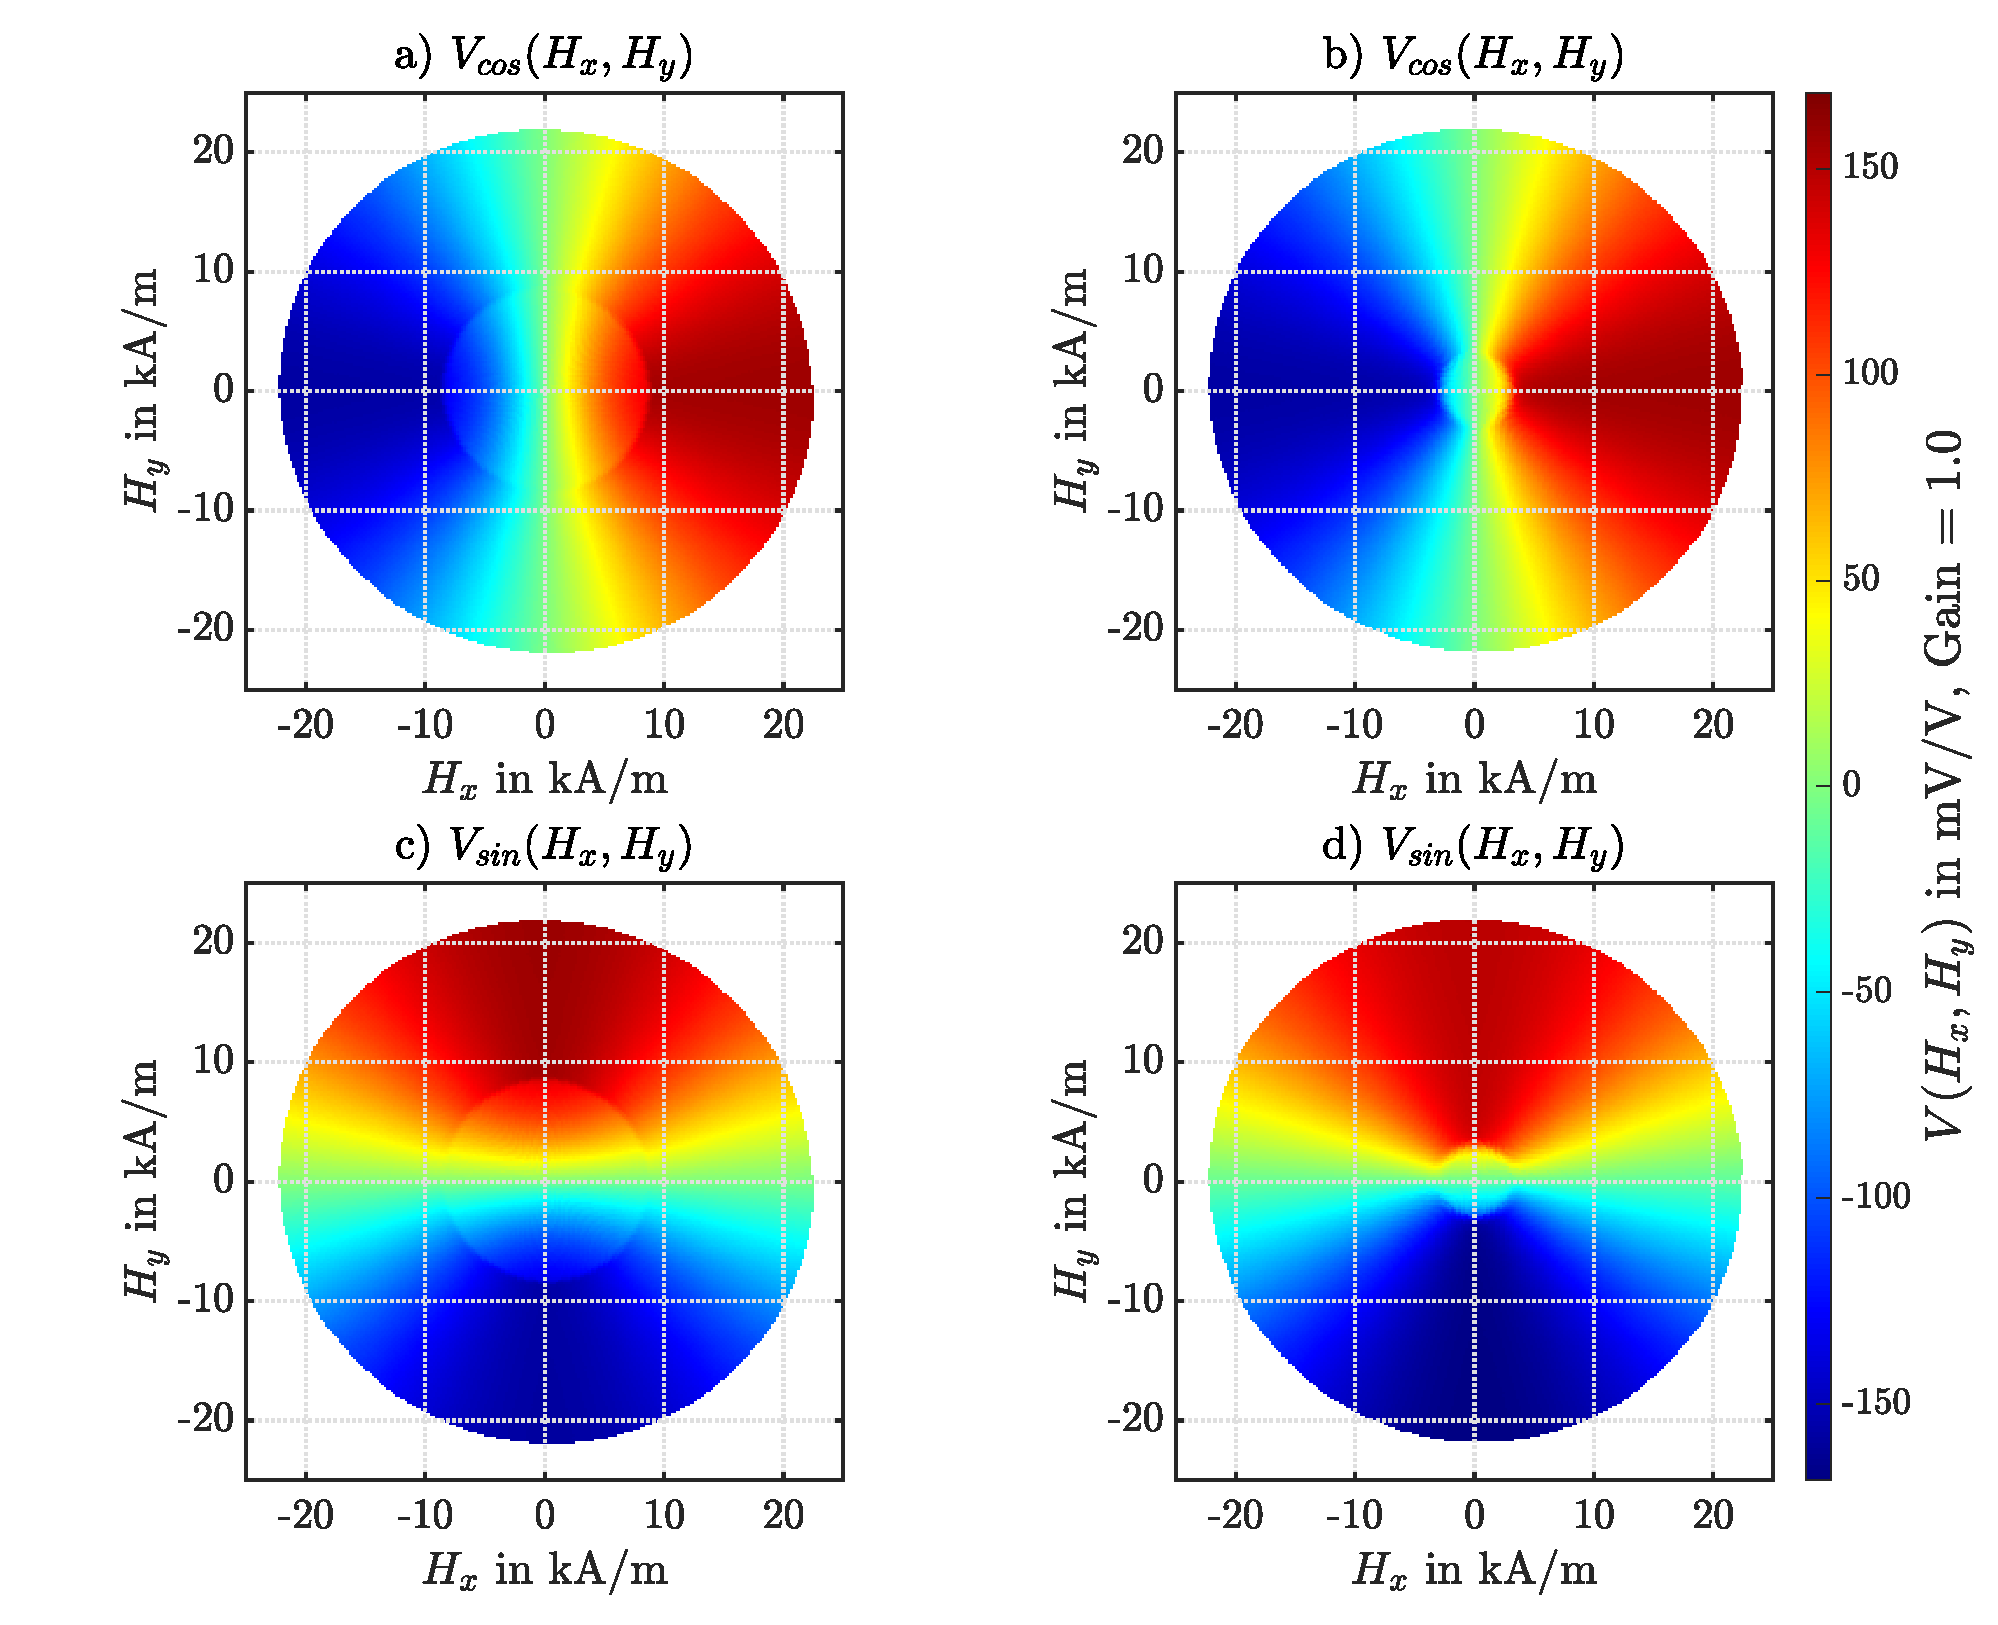
\includegraphics[width=.95\linewidth]{appendix/images/3-TDK/TDK_Kennfelder}
	\caption[TDK TAS2141-AAAB Brückenkennfelder]{TDK TAS2141-AAAB Brückenkennfelder. Kennfelder der Cosinus-Brücke a) 
		und b). Kennfelder der Sinus-Brücke c) und d). a) und c) gewonnen aus steigenden Amplitudenmodulation. b) und 
		d) gewonnen fallenden Modulation. Die Kennfelder sind normiert in $\SI{}{\milli\volt\per\volt}$. Grafik 
		nachempfunden 
		aus \cite{Schuethe2019}.}
	\label{fig:tdkkennfelder}
\end{figure}


\clearpage


Im Vergleich der Kennfeldpaare biete sich das erste aus aus \autoref{fig:tdkkennfelder} a) und c) für eine Simulation 
an. Die Kennfelder besitzen größere Plateauflächen \cite{Schuethe2019}. In \autoref{fig:tdkkennfeldsteigend} a) und c) 
ist das Kennfeldpaar nochmals gesondert dargestellt. Für das Kennfeld, der Cosinus-Wheatstone-Brücke in a), sind 
Querschnitte für variable $H_x$- und verschieden konstante $H_y$-Feldstärken in b) aufgetragen. Das gleiche vice versa 
in d) für Sinus-Wheatstone-Brücke aus c). Die Plateau-Grenzen liegen in $H_x$- und $H_y$-Richtung ca. bei 
$\pm\SI{8,5}{\kilo\ampere\per\metre}$ und sind als Limits in \autoref{fig:tdkkennfeldsteigend} b) und d) 
gekennzeichnet. Es zeigt sich ein annähernd linearer Bereich für die Übertragungskennlinien bei $H_{x,y} 
= \SI{0}{\kilo\ampere\per\metre}$. Dieser Arbeitsbereich ist für die Simulation einzustellen \cite{Schuethe2019}.


\vspace{5mm}
\begin{figure}[bph]
	\centering
	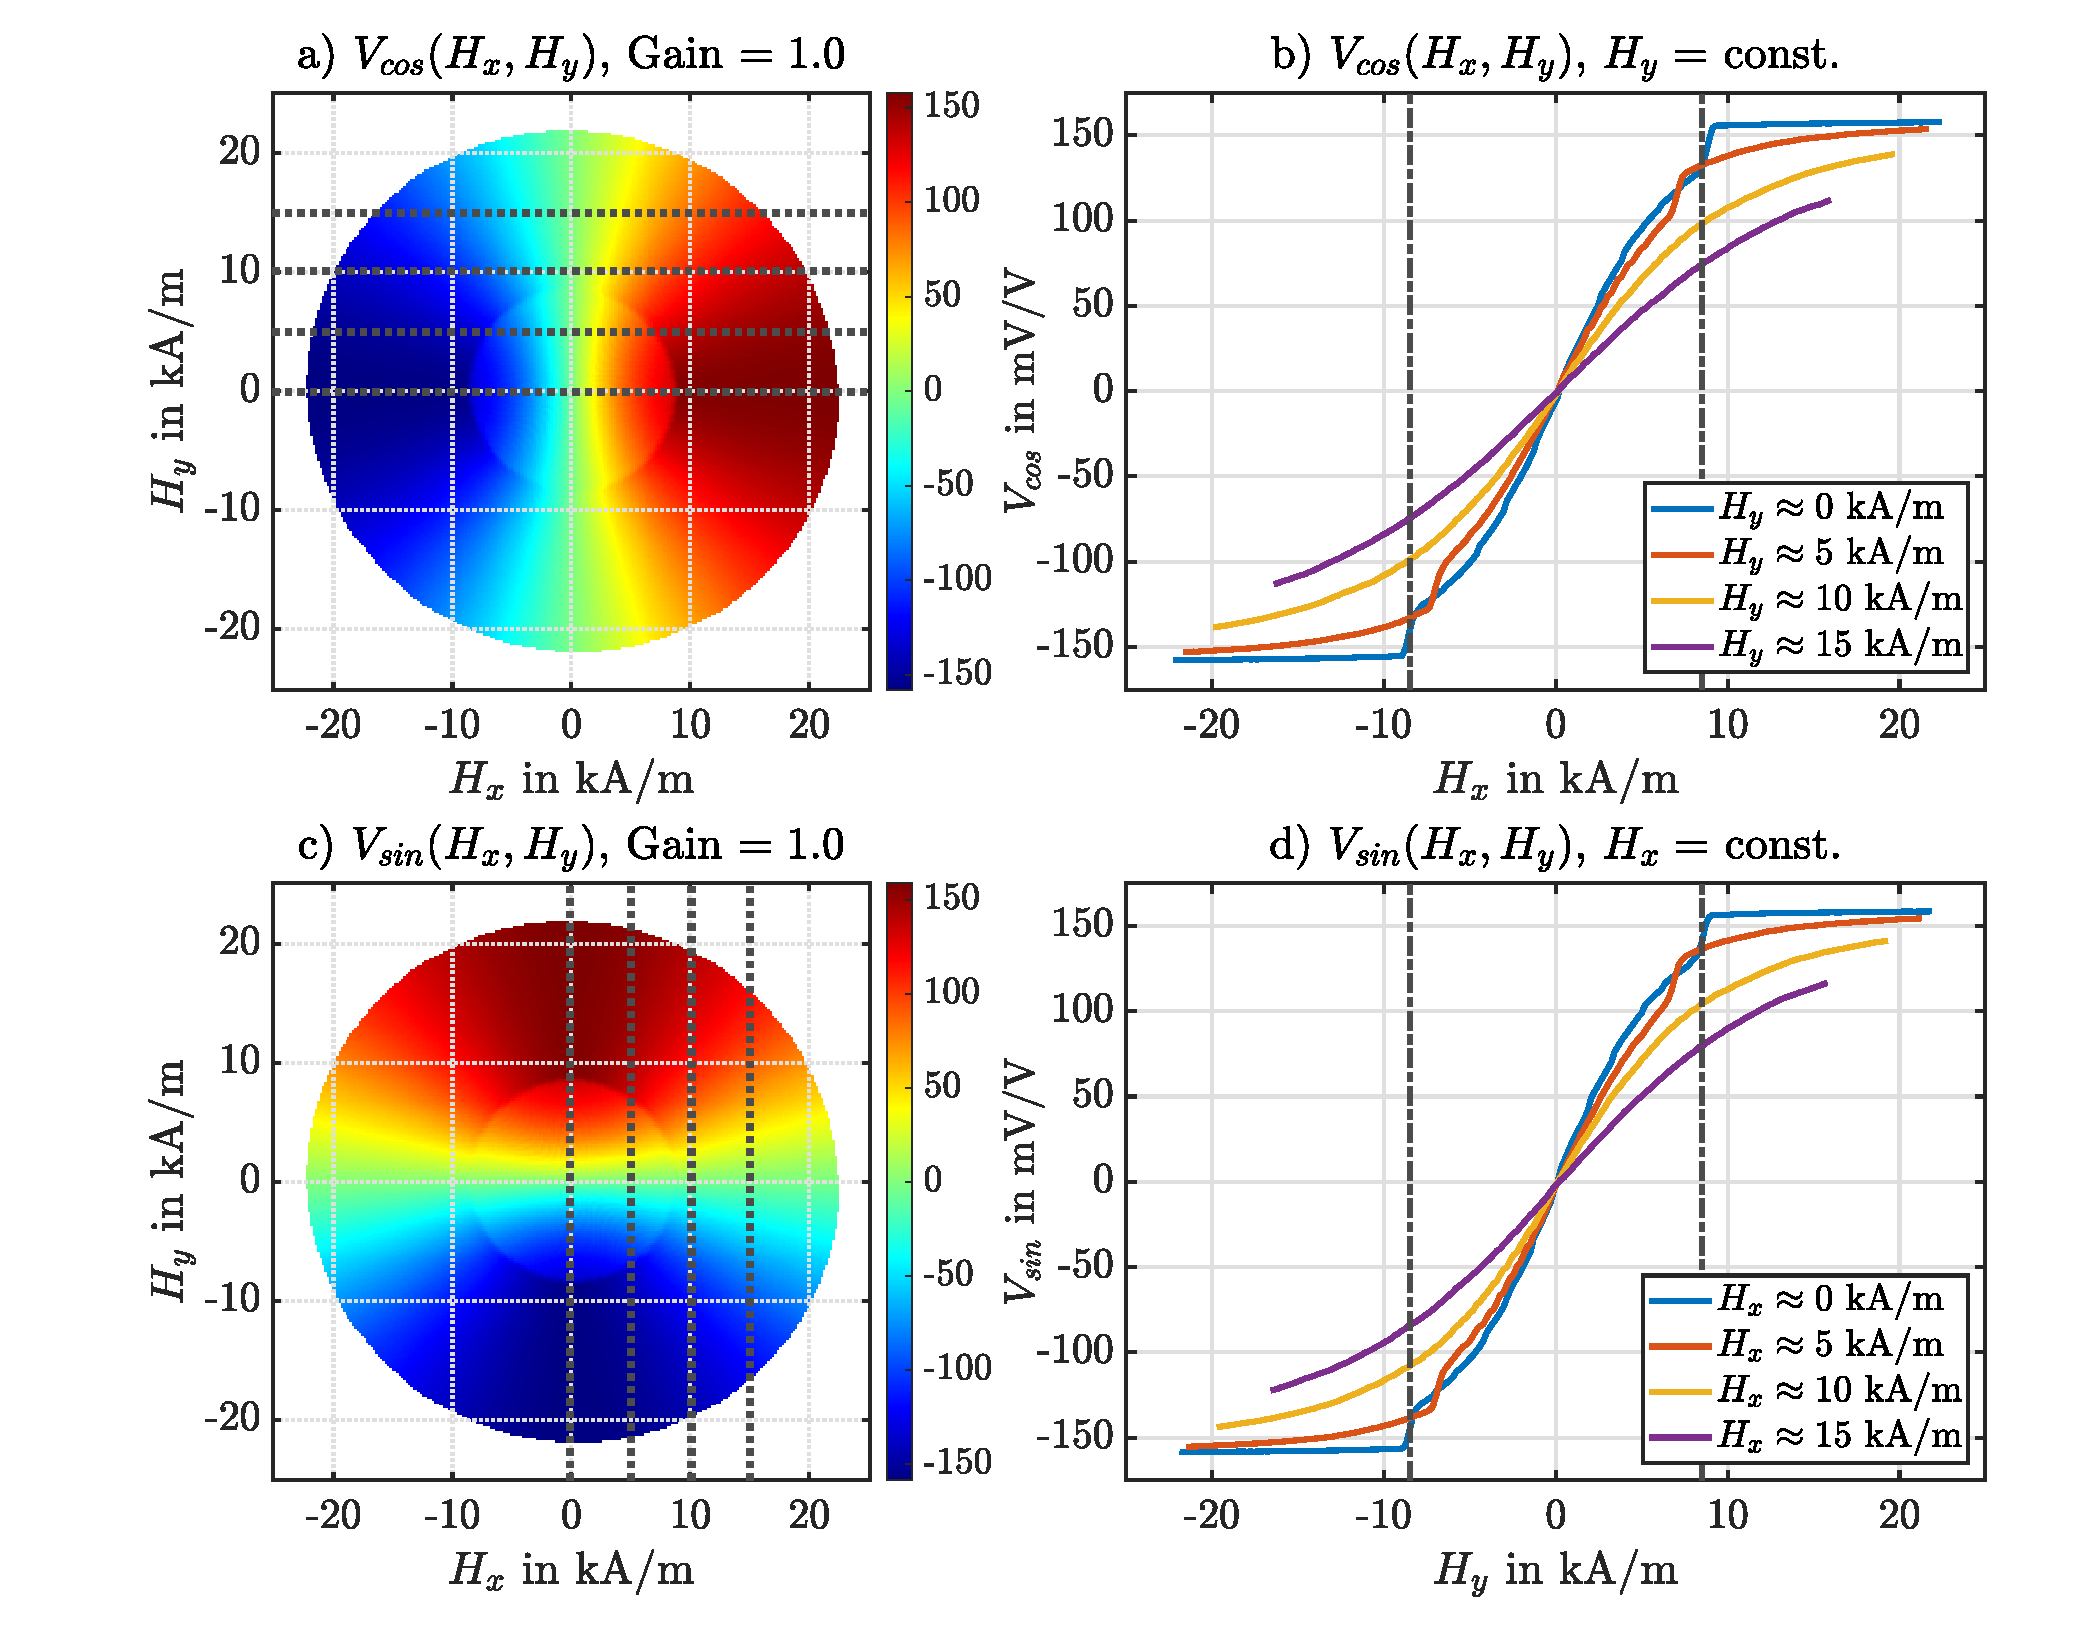
\includegraphics[width=.95\linewidth]{appendix/images/3-TDK/TDK_Kennfeld_Steigend}
	\caption[TDK TAS2141-AAAB Kennfeldquerschnitte]{TDK TAS2141-AAAB Kennfeldquerschnitte. Cosinus-Brücken-Kennfeld in 
	a) und Sinus-Brücke in c). In b) und d) sind folgend der Verdrehung Querschnitte aus a) und c) aufgetragen. In b) 
	$V_{cos}$ f. variable $H_x$- und verschieden konst. $H_y$-Feldstärken. In d) vice versa für $V_{sin}$ mit 
	verschieden konst. $H_x$- bei variablen $H_y$-Feldstärken. Breite lineare Plateaus liefern einen annähernd linearer 
	Arbeitsbereich in c) und d) zw. $\pm\SI{8,5}{\kilo\ampere\per\metre}$ f. Übertragungskennlinien $H_{x,y} = 
	\SI{0}{\kilo\ampere\per\metre}$. Grafik aus \cite{Schuethe2019}.}
	\label{fig:tdkkennfeldsteigend}
\end{figure}
